\section{Discussion}

\vspace*{1cm}

Modeling and predicting forest ecosystem dynamics is critical to anticipate and mitigate the impacts of climate change. 
However, little is known about the relative performance of correlative and process-explicit approaches. In particular, it is unclear whether there is a "quantifiable" advantage in taking the time to develop and use complex models. We believe that this work has provided important insights to better understand how model forecasts can be improved. This is a crucial step to make ecology more relevant to policy makers \citep{Dietze2017}.

In Chapter 1, we proposed and tested an optimization method to leverage high computational resources for calibrating process-explicit models with the same data as correlative models. This was one of the technical hurdles of this PhD thesis because we were uncertain, initially, which method to use and to what extent this calibration was really feasible. Overcoming this hurdle allowed us to develop an intermediate modeling approach (\emph{fully data-driven} process-explicit models). This was an essential step for Chapter 2, in order to precisely understand what promotes model robustness. It also allowed us to suggest avenues to promote the use of process-based models, which we discussed in more detail in Chapter 3.

Chapter 2 represents the largest effort of this PhD thesis. We had to process the climatic data, which is a relatively straightforward step when using correlative models (which are based on monthly variables), but becomes much more complex when using process-based models (which require daily variables). We also had to adapt a relatively simple migration model, so we could compare model projections with fossil pollen data. All of this allowed us, for the first time, to compare a range of different SDM approaches (CSDM, fitted PEM, PEM) under novel climatic conditions and disentangle the potential drivers of model transferability. Importantly, we demonstrated that describing biological processes explicitly should increase our confidence in extrapolating beyond the current extent of climatic conditions. 

Interestingly, we also found that fitted PEMs -- despite being calibrated with species distribution data -- were still relatively reliable 12,000 years ago. We thus wanted to delve deeper into this aspect in Chapter 3, in order to understand what inverse calibration entails in terms of realistic processes. By comparing PEM's prediction of phenological traits to phenological observations, we demonstrated that blindly trusting parameter estimates obtained with inverse calibration and assuming that the structural constraints of process-explicit equations are sufficient to obtain realistic estimates would be misleading. There is no miracle solution for spreading the use of process-explicit models, but we showed nevertheless that a thoughtful application of inverse calibration can still help obtain more realistic parameter values, yielding better results at the European scale.

Finally, in Chapter 4, we used these models to produce projections of species range shifts in the future using different climate projections. In particular, we paid close attention to characterizing and quantifying the different sources of uncertainty -- which is often largely ignored in favor of an appealing message. In particular, ignoring the uncertainties related to the different modeling approaches could significantly alter the implications for forest managers, especially since the use of correlative models is a subject of debate.

In the following, I will discuss:
\begin{itemize}
\item the implications and limits of our findings,
\item the main pitfalls in using process-based models,
\item  and the potential perspectives for improving them.
\end{itemize}

\subsection{General discussion of the results}

\subsubsection{Efforts to model processes explicitly  may improve model transferability}

Our comprehensive assessment of model transferability over the last 12,000 years leads us to believe that a process-explicit structure is essential for enhancing model performance, contributing to a greater model robustness to major climate changes. At the end of the Pleistocene/beginning of the Holocene, process-based models appeared better at predicting climate refugia -- locations where species could have survive under very different climatic conditions.
This was true for both classic process-explicit models (whose parameter values do not depend on the current distribution) and fitted process-explicit models, calibrated in the same way as correlative models. We thus demonstrated for the first time that there is a real benefit, to improve model transferability, in making the effort to translate our knowledge into mathematical equations by assuming cause-to-effect relationships. 

Looking at the projected migration routes of the different species in details gave more insights on the model ability to reproduce what is believed to have occurred since the Last Glacial Maximum. For instance, projections of the distribution of \emph{Fagus sylvatica} over the Holocene with PHENOFIT-fitted did not agree perfectly with the best-guess scenario based on fossil and genetic data (\Cref{fig:migration}; \citealp{Magri2006}). Overall, the projections confirmed that the postglacial spread of beech was continuous through Europe. In agreement with \citet{Magri2006}, the model projected the presence of several populations of beech in the eastern Alps–Slovenia–Istria region that could have played an important role in the colonization of Central Europe (\Cref{fig:migration}). The model  also projected many potential refugia along the eastern Adriatic coast, but not further south in Greece. PHENOFIT-fitted did not projected any refugia in Southern Italy or in the Basque Mountains. These populations, however, are not believed to have contributed to the colonization of the rest of Europe. For example, southern Italy populations likely never reached the northern part of Italy \citep{Magri2006}. The model also missed an important refugium in the Western Alps (\Cref{fig:migration}). One explanation could be that the coarse scale of the simulations did not capture the microclimatic conditions that might have favored the local persistence of beech populations. Interestingly, the model projections confirmed the presence of beech microrefugia in south-western France \citep{Lafontaine2014}, that were not mentioned by \citet{Magri2006}. The projections further suggest that these populations could have contributed to the spread of beech in France and in the Pyrenees.

\begin{figure}[h]
\centering
\includegraphics{discussion/figs/fagus_migration.pdf}
\caption{\textbf{Comparison of beech migration as simulated by PHENOFIT-fitted (left) and the migration scenario described in \citet{Magri2006} (right).} In the left plot, the color scale indicates the potential date of arrival, from earlier colonization (yellow) to later colonization (blue). Orange areas represent the potential refugia -- used as starting points for the migration model. Red crosses indicate the refugia mentionned by \citet{Magri2006} that were not simulated by PHENOFIT fitted.}
\label{fig:migration}
\end{figure}

\subsubsection{The parameter burden} 
\label{sec:parameter}

The advantage of process-explicit models also lies in the fact that we can evaluate the realism of all the intermediate processes and associated parameters, and not just compare the higher-level output to distribution data. When we make this effort, it allows us to delve deeper into the results obtained and take a step back. Large-scale inverse calibration can lead to processes that are totally unrealistic. For example, we can obtain significant errors in phenological processes, and thus lose the inherent benefits of PEMs.
This is a significant pitfall, which could become widespread given the growing popularity of process-explicit models and the increasingly easy access to powerful computing clusters.  Inverse calibration of PEMs requires extra care.
An example that struck me is the case of TTR-SDM \citep{Higgins2012}. This model is process-explicit, even though the effects of monthly climate variables are only accounted for through empirical relationships. The model is calibrated using an optimization algorithm with species distribution data. To our knowledge, the 18 parameters of the model have never been measured in a laboratory, which prevents a true assessment of their value. TTR-SDM appears better than a correlative model to predict Australian eucalypt and \textit{Acacia} species distribution outside Australia \citep{Higgins2020}. This comparison seems to be sufficient to then justify the use the model for projecting the distribution of more than 135,000 species under future climate conditions \citep{Conradi2024}. 

Without questioning the interest or the validity of the results, it seems important to have a critical look at the processes simulated by a PEM calibrated with distribution data only. We have shown that a process-explicit structure alone is not a sufficient constraint during the inverse calibration and does not prevent from reproducing the same biases as correlative models. In our case, if we had not made the effort to evaluate individual processes in Chapter 3, one could have concluded from Chapter 2 alone that a fitted PEM would necessarily give reliable projections in the future, and that it could be calibrated for any tree species of interest. Moreover, a fitted PEM may produce projections that are overly pessimistic (Chapter 4). Therefore, parameter estimation must remain a critical point of vigilance. It is all the more true that changing a single parameter value can significantly impact the simulations. For instance, increasing frost tolerance in beech, as motivated by the results from Chapter 3, leads to major changes in the fitness simulated by PHENOFIT (\Cref{fig:updatedparam}).

\begin{SCfigure}[][h]
\centering
\includegraphics{discussion/figs/updatedparam.pdf}
\caption{\textbf{The impact of one parameter value at the European scale.} The frost hardiness was changed from -20\degree C to -33\degree C based on the results of Chapter 3. Color scale indicates the fitness, from 0 (light red) to 1 (dark blue).}
\label{fig:updatedparam}
\end{SCfigure}

Interestingly, the recent trend to refine correlative models relies on the integration of more precise data (e.g. measured physiological parameters, \citealp{Kuo2022}) -- rather than on trying to calibrate complex mechanistic relationships only from species distribution data. \citet{Wagner2023} used laboratory-derived thermal performance curves to inform CSDM, for three freshwater fish species. The approach was then further developed to jointly model several species, taking into account how they depend on each other in a Bayesian framework where 
prior distributions on thermal response parameters were derived from literature values \citep{Custer2024}. For tree species, {\color{um-red} Baranger et al.} ({\color{um-red}2024}, in review) used physiological tolerance traits for frost and drought (from literature and additional measurements) to derive the distribution of 38 European tree species\footnote{A. Baranger and I are currently supervising an intern to compare this modeling approach with PHENOFIT, but the work is not yet advanced enough to be presented here.}. It thus seems overly optimistic to think that we could realistically apply process-explicit approaches to a large number of species by omitting these parametrization constraints and calibrating them only with distribution data.

\subsubsection{What does "being robust" really mean?}

The fact that the fitted PEM appears fairly accurate in the distant past despite simulating unrealistic processes highlights that it is possible to achieve correct outcomes for the wrong reasons, even in very different climatic conditions. This is something known for statistical models, where the wrong model can sometimes give better predictions than the correct one \citep{Hagerty1991, Shmueli2010}. Here, we have shown that PEMs may also reproduce observed patterns with success (e.g. past species distribution) without necessarily simulating the true mechanisms that cause them. Obviously, a good fit to data does not necessarily mean that the model is correct, as there is no "\emph{transfer of truth from data to models}" \citep{Gramelsberger2020}.

Our paleo-evaluation is also highly context-specific. We evaluated the models using a small number of species, opportunistic fossil data, a single climate model, and a single migration model. Moreover, the conditions during the Holocene were different from the conditions that are expected in the future (\Cref{fig:analog}) and one would need to go back much further in time to find analog conditions \citep{Burke2018, Tierney2020}, which is not really feasible. For all these reasons, we have chosen not to apply different weights to each model for future projections.  

\begin{figure}[h]
\centering
\includegraphics{discussion/figs/tierneyetal2020.pdf}
\caption{\textbf{Past and future climatic conditions, adapted from \citet{Tierney2020}}. Climate are colored by their global mean temperature change relative to preindustrial conditions, ranging from blue (colder) to red (warmer).}
\label{fig:analog}
\end{figure}

I believe that the value of process-based models extends beyond a specific value of a specific metric of evaluation that might be higher than another modeling approach. Process-based models represent a significant advancement in our ability to understand and simulate the dynamics of ecosystems \citep{Pilowsky2022}. Efforts to integrate current scientific knowledge into explicit mathematical formulations appear to be the way forward in science \citep{Evans2012}. It allows for clear hypothesis formulation, distinguishing between relevant and irrelevant features. A robust model is, therefore, primarily one that should appropriately represent the current state of scientific knowledge in alignment with our scientific purpose -- i.e. capturing the essential processes at the spatiotemporal scale of interest \citep{Gramelsberger2020}.

\subsubsection{Implications for ecosystem management in a uncertain world}

As perfectly summarized by \citet{Dawson2011}, "\emph{the heavy reliance of conservation management and policy on a single scientific approach creates risks of policy or management failures, particularly given that the underlying assumptions of that approach are under debate}". Indeed, we have shown that the discrepancies between the different modeling approaches we considered represent a significant share of the uncertainties of future species range shifts (\Cref{fig:cascadebonus}). Researchers may omit some uncertainties because they believe communicating on them can have a negative effect on public trust \citep{Howe2019, Simmonds2024} and may prefer to deliver what they consider a clear message -- sometimes to favor the publication of their results in a competitive academic world \citep{Yao2023}. However, this is a poor strategy because it may decrease public support for science in the long term, particularly if exaggerated pessimistic projections do not ultimately occur \citep{Kreps2020}. Expressing uncertainties may indeed have constructive effects on scientists' credibility, and increase the number of people more supportive of initiatives to tackle climate change \citep{Howe2019}. Importantly, ignoring these uncertainties may also lead to poor management decisions \citep{Simmonds2024}. It could favor intensive intervention strategies (e.g. introduction of species outside their native range), while it might be possible to rather enhance the forest's genetic adaptive capacity. Quantifying and communicating uncertainties -- including by integrating different modeling approaches -- is one of the way to make ecological modeling more relevant to decision making \citep{Dietze2017, Saltelli2020}. 

\begin{figure}[H]
\centering
\includegraphics{discussion/figs/cascade_bonus.pdf}
\caption{\textbf{The cascade of uncertainties in beech future range shift projections, considering (a) only correlative models and (b) all models (\hyperref[chapter4]{Chapter 4})}. Each individual calibrated model (i.e. 4 different CSDMs, 100 fitted PEM parameter sets, 10 partially fitted PEM parameter sets, and 1 expert PEM parameter set) was run with the 5 different GCM climatic variables (i.e. 20 CSDM projections, 500 fitted PEM projections, 50 part. fitted PEM projections, and 5 expert PEM projections). Then, they were averaged at the GCM-level within each SDM approach ("\emph{GCMs multi-calibration means}"), then averaged at the level of the SDM approach ("\emph{SDMs multi-GCM means}"), and finally further averaged at the SSP-level ("\emph{SSPs multi-SDM means}"). Note that this figure is directly inspired by \href{https://www.ipcc.ch/report/ar6/wg1/figures/chapter-1/figure-1-15}{one figure} in the IPCC AR6 report.}
\label{fig:cascadebonus}
\end{figure}


\subsection{Process-explicit modeling: are we on the right track?}

\subsubsection{The accumulation of layers can undermine model reproducibility}

As noted by John D. Aber few months after I was born, "\emph{we allow far more hand-waving in the presentation of modeling results than we do for experimental data}" in ecology, which makes the models easier to criticise \citep{Aber1997}. The accumulation of successive layers in the development of models indeed poses significant challenges to scientific transparency and reproducibility. 

Models often draw inspiration from each other. This practice is fundamental in the development of science: we build upon previous results to add new insights or adapt the model to another context \citep{Bugmann2022}. However, it may also lead to the propagation of errors or unjustified parameters. For instance, in the JABOWA model \citep{Botkin1972}, the mortality rate of slow-growing trees was set to $0.368$ for all species (based on an arbitrarily established survival rate of 0.01 in 10 years; \citealp{Kobe1995}). This value was then used in several gap models: FORECE \citep{Kienast1987}, ForClim \citep{Bugmann1996}, and today in ForCeeps \citep{Morin2021}. This can lead to potential errors if the parameter value is not suited to the specific modeling context. Furthermore, in a multi-model ensemble, this may bias projections towards similar models and lead to an underestimation of uncertainties \citep{Pathak2023}.

As models evolve, researchers often adjust and integrate new relationships and parameters to improve predictions' accuracy. 
The lack of clear justification behind each choice can make it difficult to discern the underlying logic of the multi-layered structure \citep{Harrison2021}. The introduction of new layers may also involve making assumptions that are not always thoroughly validated. There is often a strong \emph{connection} between the researcher and their model \citep{Dahan2009}, and they intuitively feel what kinds of adjustments could be useful for achieving certain goals \citep{Gramelsberger2020}. These choices are often interconnected, and it can be hard, from an external perspective, to understand the origin of each aspect and from which assumption it is derived \citep{Gramelsberger2020}. Some decisions made in the past may no longer be optimal today, for example the programming language chosen decades ago may no longer be adapted to the greater computational power available today. Rigorous documentation practices should enhance the reproducibility and overall credibility of models. However, implementing them becomes more challenging once the model has been developed for many years -- although some PhD students or postdocs may be brave enough to do so \citep{PetitCailleux2020}, but it was not my case. Today, however, codes are becoming increasingly accessible and the use of models is facilitated, notably through R packages (e.g. TROLL model \citep{Schmitt2023}, \href{https://gitlabext.wsl.ch/boehmd/treemig}{TreeMig} model).

\subsubsection{Limits to the understandability and manageability of models}

While realism, generality and precision were the main focus of \citet{Levins1966}, he also mentioned \emph{understandability} and \emph{manageability} as important criteria \citep{Levins1993}. They are part of the trade-off during model building, and we may wonder to what extent process-explicit models are still tractable when we increase complexity. 

In climatology, global climate models (GCMs) are constantly being updated and become more and more complex. For example, in the last \citet{IPCC2021} report, \emph{next-generation} models have an improved representation of clouds and aerosols, which caused a different behavior without being fully explainable \citep{Voosen2019}. The simulations of GCMs themselves have become a subject of study to disentangle all the processes modelled and understand the sensitivity of the models \citep[e.g.][]{Zelinka2020}. Thus, it might be tempting to follow the same path for ecological models. Obviously, the level of abstraction depends on the intended objective and may evolve during the course of the research. However, this is not the same spatial resolution expected as climate models (around 100 km), as in the most ideal case forest managers would want projections at the stand scale \citep{Cheaib2012}.

Increasing the complexity of PEMs may indeed hold promise for advancing our understanding of ecosystems. It seems to be a necessary step if we want to understand the intricate impacts of human activities on the various contributions of ecosystems (including forests) to human well-being, as well as all the interactions between these contributions. High-performance computing resources now allow to easily handle such complex PEMs. As an illustration, the \href{https://anr.fr/Project-ANR-21-CE32-0010}{FISSA project} proposes to knit complementary PEMs together (ForCeeps, PHENOFIT, SurEau, Yasso) to better simulate forest dynamics and functioning in order to meet the expectations of decision-makers and forest actors. The hope is that small and well-understood models can be coupled, and that their good performance will extend to the whole. An other avenue could be the hybridisation of machine-learning method and process-explicit model. It has recently gained a lot of attention in climatology \citep[e.g.][]{IglesiasSuarez2024}, and could be adapted in ecology to develop realistic models with improved interpretability and minimal computational cost.

However, increasing complexity also presents challenges. The inclusion of more processes generally involves additional parameters. Even if each of them are accurately measurable, the model outcome may be less predictable \citep{Levins1993}. We may fall in a \emph{complexity trap}, where potential increase in realism are counterbalanced by "\emph{decreases in transparency, robustness, and predictive power}" \citep{Franklin2020}. To find the right amount of complexity, multiple alternative formulations within the same model architecture could be simultaneously evaluated \citep{Huber2020}. Yet, in any case, understanding the sources of uncertainty and their propagation through the model may become nearly impossible. This is a common criticism to PEMs, so we should be vigilant. Researchers indeed tend to develop PEMs with dozens of parameters without explicitly quantifying parameter uncertainty, and often neglect to propagate this uncertainty when making projections \citep{Dietze2017}. Even sensitivity analyses are rare \citep[e.g.][]{Huber2018}, as they are time-consuming and offer little scientific recognition, although they should be a prerequisite for using a model to avoid losing track of how it works. Finally, increasing model complexity may not challenge only researchers but also decision-makers who rely on model outputs, as each additional process and parameter may increase model uncertainty to the point at which predictions are not sufficiently useful \citep{Saltelli2020}.

\subsubsection{Benefiting from all the data available}

Over the past decade, the number of various large-scale data sources has increased significantly. PEMs could benefit from these new massive databases, to spread their use for many species \citep{Evans2016}. Indeed, the development of new tools for data collection will probably increase by at least an order of magnitude the amount of data available. Notably, forest structural measurements from 3D scanning (LiDAR) and multispectral and hyperspectral measurements of canopy can be combined to detect and classify individual trees with machine-learning method (\Cref{fig:autospecies}; \citealp{Maeyrae2021, Ma2024}). This automatic tree segmentation enables tracking individual trees and their phenology \citep{Berra2019}. It could also allow to better estimate the spatiotemporal variability caused by intraspecific diversity and local adaptation \citep{Randin2020}, and better understand the impacts of extreme climatic events (e.g. leading to crown defoliation). In addition to these new tools, there are also efforts to gather large-scale data, such as the PROFOUND database design specifically to calibrate and evaluate vegetation models \citep{Reyer2020}. Citizen science networks also enable the gathering of data at large scales (e.g. the \emph{Observatoire des Saisons}\footnote{\url{https://www.obs-saisons.fr/}} in France). They contribute directly to gain new scientific insights \citep[e.g.][]{Asse2018}, including by calibrating remote-sensing measurements with ground observations \citep{Xu2024}.

\begin{figure}[h]
\centering
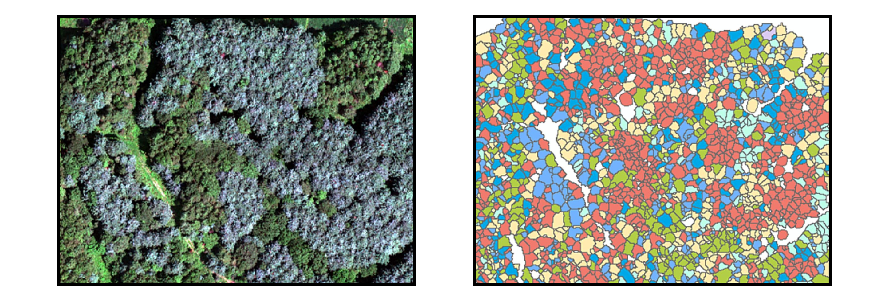
\includegraphics{discussion/figs/maetal2024.pdf}
\caption{\textbf{An example of automatic tree species classification, adapted from \citet{Ma2024}.} The classification was done using neural networks based on hyperspectral images and LiDAR data. Each color corresponds to a different species.}
\label{fig:autospecies}
\end{figure}

By integrating data across different scales and detailed understanding of mechanisms, there is a thus high potential to develop data-driven, yet still process-explicit, models. It requires to combine multi-disciplinary expertise in machine learning (to sift through data) and process-explicit modeling\footnote{This was one of the objectives discussed during \href{https://www.lorentzcenter.nl/fair-phenological-modelling.html}{a week-long workshop} in Leiden (Netherlands) around the topic of phenology, which I attended in spring 2024.}. The challenge is not just about acquiring new data -- it is also about effectively integrating them into the models. In the example of the beech frost hardiness mentioned earlier (\Cref{fig:updatedparam}), the parameter value was outdated and did not align well with recent studies. Optimization methods such as CMA-ES (Chapter 1) are critical to tune the model and find parameter values that best reproduce a chosen set of observations. The methodological framework to assimilate simultaneously various and often heterogeneous datasets is still relatively new but it receives more and more attention \citep{Zipkin2021}, including for correlative models \citep{Isaac2020}. However, there are multiple issues that may lead to biased inferences. In particular, difference in the quantity and the quality of the data may produce bias parameter values toward abundant sources regardless of their quality \citep{Zipkin2021}. Bayesian inference may offer a promising framework to combine multiple data types at different scales \citep{Hartig2012}, as each can be encoded in a likelihood function which can then combined easily (if the different sources are not correlated). For example, \citet{Cailleret2020} used forest inventory data to calibrate a growth-dependent mortality model, mixing information about basal area increment and stem numbers in one joint likelihood function (yet using non-informative priors). In our specific case, it would have been possible to implement a multi-objective CMA-ES \citep{Igel2007}, balancing the fit to distribution data with phenological observations to guide the optimization algorithm towards parameter sets that align well with both data sources.
It could have helped PHENOFIT not only to simulate accurately species distribution but also capture essential phenological processes, and reduce parameter non-identifiability issue \citep{Zipkin2021} -- at least for the species for which we have enough observations. Inverse calibration thus represents a great opportunity to coherently integrate information from many large-scale data sources -- by still making sure that the measurements correspond to the model outputs (“\emph{model what you measure, measure what you model}”; \citealp{Fisher2014}). Yet, we should keep in mind that inverse calibration may induce some compensation of the potential misconceptions and errors in the model structure and fixed parameters. Moreover, large-scale data assimilation is not effective if we lack the necessary knowledge, from intensive monitoring sites and stand-scale experimental data, to develop realistic process representations in order to reduce future projection uncertainties \citep{Keenan2012}. 

\subsection{Rethinking process-explicit models}

Two visions of future PEM development emerge:
\begin{itemize}
\item complexifying models, following the classical belief that model improvement must rely on additional processes \citep{Fisher2014}
\item focusing on the critical analysis of main asssumptions and processes to build a more robust modeling framework \citep{Harrison2021}
\end{itemize}

Neither path is inherently better than the other -- as always, it depends on the objectives and scale of interest, which determine which processes are essential and which are superfluous \citep{Bugmann2022}. Similarly to climate models, refining ecological models with new mechanisms helps understand the complexity of the ecosystem functioning and explore the boundaries of our knowledge. However, we may quickly encounter numerous unknown parameters. I have mainly focused on the first approach so far, discussing the advantages and disadvantages of process-explicit models in their current form, as well as opportunities for improvement. I believe, however, that an other path is also possible, especially for models whose aim is to make causal inferences on a large scale -- as process-explicit species distribution models (e.g. PHENOFIT). 

\subsubsection{Simplifying and clarifying the hypothesis behind the model}

It is common to consider a simplified version of a model for large-scale applications. For example, SurEau-Ecos simplify a more complex plant hydraulics model (SurEau), by limiting the number of parameters and reducing computing time \citep{Ruffault2022}. Nevertheless, it still requires a lot of data, such as detailed soil characteristics, and species-specific parameters not always available (e.g. whole-plant conductance). 

One avenue to simplify models is to look for the most parsimonious explanations. In the eco-evolutionnary optimality (EEO) framework, the idea is to make strong assumptions on the trade-offs that organisms must make, on an appropriate temporal and spatial scale \citep{Franklin2020, Harrison2021}. 
For example, an \emph{optimality} (i.e. cost-minimizing) hypothesis can be to assume that a leaf maximise carbon gain and minimise water loss (on the time scale of physiological acclimation, e.g. few weeks), in order to derive one single global equation and to reduce the number of parameters poorly constrained by observations \citep{Wang2017, Harrison2021}. It as a powerful framework for predicting plastic processes based on plant trait variations as a function of environmental conditions \citep{Franklin2020}. The goal is now to incorporate these equations into land surface models, which constitute a critical component of climate models \citep{Franks2018}. Optimality principles may also offer a promising way forward to model species range shifts \citep{MartinezVilalta2023}.
Rather than a fixed mean parameter value per species, one could consider that plastic traits should be predicted based on an optimalility theory, or at least separated in an plastic component (varying with the environment) and a non-plastic (heritable) component \citep{Franklin2020}. 

\subsubsection[Redesigning model structure from a Bayesian perspective: one ring to rule them all?]{Redesigning model structure from a Bayesian perspective: one ring to rule them all?\footnote{Many thanks to Lizzie Wolkovich to have agreed to read and give her opinion on this section.}}

So far, we have mostly contrasted statistical approaches with process-explicit ones. Even our fitted process-explicit approach is not an hybrid, as it relies only on the calibration of PEMs with the same data as correlative SDMs. Yet, we have seen that statistical models are evolving towards more mechanistic approaches. I believe the other way may also be powerful if process-explicit modelers increasingly leveraged robust statistical approaches. 

The opportunity for merging the two approaches and building more robust models has never been higher. The idea is to move away from the traditional framework of PEMs, where parameters are typically assigned single fixed values based on current knowledge or calibration to observed data. Bayesian hierarchical models could offer a rigorous framework for model fitting, parameter identification, and uncertainty quantification, and are already widespread in ecology \citep{Cressie2009, Zurell2016}. Based on our current ecological understanding, it is possible to build a mathematical narrative of how the data is generated \citep{Betancourt2020}, encapsulating both the data structure and our domain expertise. Bayesian inference could be applied to process-explicit equations to estimate parameters and quantify uncertainty. Parameters would be considered as random variables with probability distributions, which could be updated considering both prior knowledge and observed data. This probabilistic framework would also offer an opportunity to explicitly account for data-related sources of noise, and in particular for the discrepancies between what is measured and what is modeled (e.g. useful if we use remote-sensing data). 
It would also be more straightforward to integrate diverse data sources \citep{Cailleret2020, Cameron2022}. 

However, adapting a process-explicit model to a Bayesian framework represent many challenges. PEMs often include many functions that are not differentiable at some points (e.g. piecewise function with thresholds). Thus some equations would need to be fundamentally reformulated (see \citet{Betancourt2022} for a very detailed example adapted to phenological modelling). Moreover, PEMs also frequently have \emph{opaque} internal links between processes, which would have to be explicitly stated. These reformulations and clarifications would help us to target the right level of complexity and would favor a better model transparency. 
Computational challenges would also likely emerge, because of the difficulty to fully explore a high-dimensional parameter space in order to accurately characterize the posterior distribution -- but this would ultimately promote a better consideration of parameter uncertainty. Finally, data can often be more limiting than during a traditional PEM calibration, because we have to accumulate enough information to achieve a robust inference. However, "\emph{what doesn't kill us makes us stronger}": these constraints could prevent us from making biased inferences and unfounded assumptions beyond what the data can support.

\subsection{Conclusion}

Process-explicit models are a key tool to encourage a comprehensive and continuous incorporation of current scientific knowledge, expert opinion, and novel experimental data. They have the potential to provide more reliable projections in the future. The development of process-explicit approaches is thus essential for advancing our understanding of species and ecosystem functioning. In particular, they should be more represented in studies about climate change impacts, as they lead to more nuanced insights compared to simpler correlative models.

Inverse calibration can be a way forward to foster the use of process-explicit models. It can allow for refining parameter values by incorporating large-scale data, which have a significant impact on model performance.
Going further, inverse calibration with an optimization algorithm like CMA-ES could also allow to investigate potential traits adaptation under future climatic conditions. CMA-ES is indeed directly inspired by the principles of biological evolution (see Chapter 1): new parameter sets (individual traits) are generated via the recombination and mutation of previous parameter sets (parents), and the best individuals are then selected based on an objective function value (their "fitness"). 
We could therefore easily take advantage of the framework we have established, to optimize some selected traits under future climatic conditions (constraining the range of variation and the mutation strength) and identify which trait combinations are necessary for species to survive (\Cref{fig:cmaesevolution}). 

To conclude, I would like to insist that there is neither general recipe nor magic trick when using process-explicit models.
Different issues can occur from different contexts, species, and spatiotemporal scales.
Model refinement should rely not only on sophistication (i.e. adding new processes and parameters), but also on a step-by-step reassessment and reformulation of the model assumptions. Modeling is an iterative process: sharing early models and failures along the way can make modeling exercise more transparent and improve scientific communication.
There is a great opportunity to take advantage of interdisciplinary synergies to build models that are not only grounded in the current scientific understanding of the processes but also statistically robust.
I believe there are still many avenues to explore in order to find the right balance between theoretical concepts, various data sources to support them, and robust inference methods to improve uncertainty propagation.


